\documentclass[12pt]{article}
\usepackage{amsmath}
\usepackage{hyperref}
\usepackage{amsfonts}
\usepackage{amssymb}
\usepackage{graphicx}
\usepackage[table,xcdraw]{xcolor}
   \newenvironment{dedication}
        {\vspace*{6ex}\begin{quotation}\begin{center}\begin{em}}
        {\par\end{em}\end{center}\end{quotation}}

\usepackage{epigraph}


\title{\textbf{Image processing RRY025}\\ \textit{A quick reference sheet for the exam and not-so-thorough explanations
of areas not studied by the lazy engineering master student}}
\author{by Various Artists}

\begin{document}
\maketitle
\epigraph{In theory there is no difference between theory and practice. In practice there is.}{\textit{Yogi Berra}}
\newpage
\begin{dedication}
\hspace{4cm}
\vspace*{9cm}{This paper is dedicated to nobody.}
\end{dedication}
\newpage
\tableofcontents
\newpage

\section{Introduction}
	This document is done in order to describe the general concepts
	that has been covered in the course, and also provide answers to
	some common exam questions. The content is shamelessly ripped from
	various sources, which is indicated at the start of a section
	or paragraph.\\
	\\	
	Guide:
	\begin{description}
		\item[[W]] Wikipedia
		\item[[L]] Lecture notes
		\item[[E]] Exam
		\item[[B]] Course Book
		\item[[O]] Other
		\item[[P03]] Paper: Romeo et al. (2003)
        \item[[P04]] Paper: Romeo et al. (2004) 
		\item[None] Missing or anecdotal
	\end{description}
    	
\newpage
%	
%%%%%%%%%%%%%%%%%%%%%%%%%%%%%%%%%%%%%%%%%%%%%%%%%%%%%%%%%%%%%%%%%%%%%%%%%%%%%%%%%%%%%%%%%%%%%%%%%%%%%
%
\section{Noise}
	\subsection{General concepts}
	\subsubsection{What is noise?}
	
	[W] Image noise is random (not present in the object imaged) variation of brightness or
	color information in images, and is usually an aspect of electronic noise. It can be
	produced by the sensor and circuitry of a scanner or digital camera. Image noise can
	also originate in film grain and in the unavoidable shot noise of an ideal photon 
	detector. Image noise is an undesirable by-product of image capture that adds spurious 
	and extraneous information.\\
	
	The original meaning of "noise" was and remains "unwanted signal"; unwanted electrical
	fluctuations in signals received by AM radios caused audible acoustic noise ("static").
	By analogy unwanted electrical fluctuations themselves came to be known as "noise". 
	Image noise is, of course, inaudible.\\

	The magnitude of image noise can range from almost imperceptible specks on a digital 
	photograph taken in good light, to optical and radioastronomical images that are almost 
	entirely noise, from which a small amount of information can be derived by sophisticated 
	processing (a noise level that would be totally unacceptable in a photograph since it 
	would be impossible to determine even what the subject was).
	
	\subsection{Various types of noise}
	
	\subsubsection{Salt and pepper noise}
	[W] Salt-and-pepper noise is a form of noise sometimes seen on images. It presents itself as 
	sparsely occurring white and black pixels. An effective noise reduction method for this 
	type of noise is a \textbf{median filter} or a morphological filter. For reducing either salt 
	noise or pepper noise, but not both, a contraharmonic mean filter can be effective.
	\begin{figure}[h!]
		\centering
		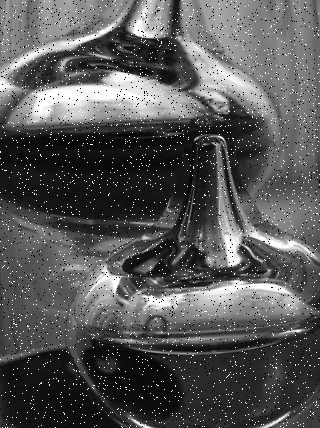
\includegraphics[width=0.5\textwidth]{img/Noise_salt_and_pepper.png}
		\caption{Example of salt and pepper noise}		
		\label{fig:salt_and_pepper}
	\end{figure}
	
	\subsubsection{Gaussian noise}
	[W] Gaussian noise is statistical noise having a probability density function (PDF) equal to 
	that of the normal distribution, which is also known as the Gaussian distribution. In other
	words, the values that the noise can take on are Gaussian-distributed.

	\begin{figure}[h]
		\begin{equation}
			p(z) = \frac{1}{\sqrt{2 \pi \sigma} }   e^{-(z - \overline{z}) / 2 \sigma^2 }
		\end{equation}
		$z$ represents the instensity \\
		$\overline{z}$ is the \textit{mean}(avrage) \\
		$\sigma$ is \textit{standard diviation} \\
		$\sigma ^2$ is called \textit{variance} \\
		approx $70\%$ of noise in range $[\overline{z} - \sigma, \overline{z} + \sigma]$ \\
		approx $95\%$ of noise in range $[\overline{z} - 2\sigma, \overline{z} + 2\sigma]$ \\
		\caption{pdf of Guassian noise, [B]	page 336}
		\label{GuassianPDF}
	\end{figure}
	
	\subsubsection{Rayleigh noise}
	Shape of the probability distrubution is slightly skewed to the right. Usefull for approximate skewed histograms.

	\begin{figure}[h!]
		PDF is given by:
		\begin{equation}
			p(z) = \left\{ 
			  \begin{array}{l l}
			    \frac{2}{b}(z - a)e^{(z-a)^2 /b} & \quad \text{for $z \geq a$} \\
			    0 & \quad \text{for $z < a$} 
			  \end{array} \right.
		\end{equation}
		Mean and variance are given by
		\begin{equation}
			\overline{z} = a + \sqrt{\pi b/4}
		\end{equation}
		$z$ represents the instensity \\
		\caption{pdf of Rayleigh noise noise, [B]	page 336}
		\label{RayleighPDF}
	\end{figure}
	
	\subsubsection{Poissonian noise}
	[W] Shot noise or Poisson noise is a type of electronic noise which originates from the 
	discrete nature of electric charge. The term also applies to photon counting in optical 
	devices, where shot noise is associated with the particle nature of light.\\
	\\
	For large numbers the Poisson distribution approaches a normal distribution, typically 
	making shot noise in actual observations indistinguishable from \emph{true Gaussian noise} 
	except when the elementary events (photons, electrons, etc.) are so few that they are 
	individually observed. Since the standard deviation of shot noise is equal to the square 
	root of the average number of events $N$, the \emph{signal-to-noise} ratio (SNR) is given by:
    $$
    \mathrm{SNR} = \frac{N}{\sqrt{N}} = \sqrt{N}
    $$
    Thus when $N$ is very large, the signal-to-noise ratio is very large as well, and any 
    \emph{relative} fluctuations in $N$ due to other sources are more likely to dominate over 
    shot noise. However when the other noise source is at a fixed level, such as thermal noise, 
    increasing $N$ (the DC current or light level, etc.) can sometimes lead to dominance of 
    shot noise nonetheless.
    
    \textbf{not additive.} \\
	\textbf{corraleted with the image.} \\
	
	Note: A \textit{poissonian distrubution} is like a Guassian distrubution when the mean is low, $\mu < 10$.
	
	\subsubsection{Additive}
    
    Additive because it is added to any noise that might be intrinsic to the information system.
	
	\subsubsection{Multiplicative}
	In signal processing, the term multiplicative noise refers to an unwanted random signal that 
	gets multiplied into some relevant signal during capture, transmission, or other processing.
	Taking $\log{f{z} + \epsilon}$ makes \textit{multiplicativ} noise \textit{additive}
	Obs, when taking $\log$ of an image, the \textit{flux} is not conserved. It can be conserved if \textit{flux} is calculated in original first, then
	
	\subsubsection{Exponential}
    The $a$ parameters controls the ammount of spread. Higher thevalue faster the function falls to zero     from the maximum. As in the case on page 316 the PDF of output image is obtained by convolution of input image     and uniform noise PDF.
	
	\subsubsection{Speckle noise}
	Uniform, multiplicative noise.
	Uncorralated to the image. Can be removed by \textit{Wiener filtering} since it can be made \textit{additive} by using the logarithm and it's uncoralated with the image.

	
	\subsection{Colors of noise}
	\subsubsection{White noise}
	[W] White noise is a signal (or process), named by analogy to white light, with a flat frequency
	spectrum when plotted as a linear function of frequency (e.g., in Hz). In other words, the signal 
	has equal power in any band of a given bandwidth (power spectral density) when the bandwidth is 
	measured in Hz. 
	\subsubsection{Pink noise}
	TODO
	\subsubsection{Blue noise}
	[W] In computer graphics, the term "blue noise" is sometimes used more loosely as any noise with 
	minimal low frequency components and no concentrated spikes in energy. This can be good noise for dithering.
	
	\subsubsection{Gamma (Erlang-noise)}
	Book page: 315-316
	
%	
%%%%%%%%%%%%%%%%%%%%%%%%%%%%%%%%%%%%%%%%%%%%%%%%%%%%%%%%%%%%%%%%%%%%%%%%%%%%%%%%%%%%%%%%%%%%%%%%%%%%%
%	
\section{Filters}
	
	\subsection{Median filter}
	\subsubsection{Description}
	[W] In signal processing, it is often desirable to be able to perform some kind of noise 
	reduction on an image or signal. The median filter is a nonlinear digital filtering 
	technique, often used to remove noise. Such noise reduction is a typical pre-processing 
	step to improve the results of later processing (for example, edge detection on an image). 
	Median filtering is very widely used in digital image processing because, under certain 
	conditions, it preserves edges while removing noise.
	
	\subsubsection{Algorithm description}
	[O] Like the mean filter, the median filter considers each pixel in the image in turn and 
	looks at its nearby neighbors to decide whether or not it is representative of its surroundings.\\
	\\
	Instead of simply replacing the pixel value with the mean of neighboring pixel values, it replaces 
	it with the median of those values. The median is calculated by first sorting all the pixel values 
	from the surrounding neighborhood into numerical order and then replacing the pixel being considered 
	with the middle pixel value. (If the neighborhood under consideration contains an even number of 
	pixels, the average of the two middle pixel values is used.)\\
	\\
	\textbf{Why use median instead of mean:}
	\begin{itemize}
	
	\item The median is a more robust average than the mean and so a single very unrepresentative pixel
	in a neighborhood will not affect the median value significantly.

    \item Since the median value must actually be the value of one of the pixels in the neighborhood, 
    the median filter does not create new unrealistic pixel values when the filter straddles an edge. 
    For this reason the median filter is much better at preserving sharp edges than the mean filter. 
	\end{itemize}

	\subsection{Mean/Averaging filter}
	[O] The idea of mean filtering is simply to replace each pixel value in an image with the 
	mean (`average') value of its neighbors, including itself. This has the effect of eliminating 
	pixel values which are unrepresentative of their surroundings.\\
	\\	
	\textbf{Problems with mean filtering:}
	\begin{itemize}
		\item A single pixel with a very unrepresentative value can significantly affect 
		the mean value of all the pixels in its neighborhood. 
		\item When the filter neighborhood straddles an edge, the filter will interpolate 
		new values for pixels on the edge and so will blur that edge. This may be a problem
		if sharp edges are required in the output. 
	\end{itemize}
	Both of these problems are tackled by the median filter, which is often a better filter 
	for reducing noise than the mean filter, but it takes longer to compute. 

    \subsection{Wiener-filter (Minimum-mean-square-error filter)}
    Wiener filter is founded on considering images and noise as random variables.
    The objective is to find an estimate, e, of the uncorrupt image, i, such that the means square error between them is minimized. 
    
%	
%%%%%%%%%%%%%%%%%%%%%%%%%%%%%%%%%%%%%%%%%%%%%%%%%%%%%%%%%%%%%%%%%%%%%%%%%%%%%%%%%%%%%%%%%%%%%%%%%%%%%
%	
\section{Image sharpening}
	The Basic concept is as follows:\\
	Sharpened image = Original image - smoothened image.\\
	You can smoothen an image by applying a lowpass filter on it.
	
	\subsection{Edge detection}
	A lot of different ways. One basic approach for finding edges is by detecting changes in intensity, 
	which can be accomplished using first or second order derivatives. \\
	
	\noindent [W]	There are many methods for edge detection, but most of them can be grouped into two categories, 
	search-based and zero-crossing based. The search-based methods detect edges by first computing a measure 
	of edge strength, usually a first-order derivative expression such as the gradient magnitude, and then 
	searching for local directional maxima of the gradient magnitude using a computed estimate of the local 
	orientation of the edge, usually the gradient direction. The zero-crossing based methods search for zero
	crossings in a second-order derivative expression computed from the image in order to find edges, usually 
	the zero-crossings of the Laplacian or the zero-crossings of a non-linear differential expression. As a
	pre-processing step to edge detection, a smoothing stage, typically Gaussian smoothing, is almost always applied.\\
	\\
    The edge detection methods that have been published mainly differ in the types of smoothing filters that are applied and the way the measures of edge        strength are computed. As many edge detection methods rely on the computation of image gradients, they also differ in the types of filters used for          computing gradient estimates in the x- and y-directions.
	
	\subsection{High Boosting}
	[B] High-boost filtering is used for sharpening an image $f(x,y)$. It is carried out in several steps, 
	namely:
	\begin{itemize}
	\item Unsharp masking \begin{enumerate}
	                        \item Blur the original image $\rightarrow \hat f(x,y)$
	                        \item Subtract the blurred image from the original 
	                        (yielding a mask) $ \rightarrow g_{\mathrm{mask}}(x,y) = f(x,y) - \hat f(x,y)$
	                        \item Add the mask to the original $ g(x,y) = f(x,y) + k * g_{\mathrm{mask}}(x,y)$
	                       \end{enumerate}
	\item If $ k > 1$ this will yield a high boosted image.
	\end{itemize}
%	
%%%%%%%%%%%%%%%%%%%%%%%%%%%%%%%%%%%%%%%%%%%%%%%%%%%%%%%%%%%%%%%%%%%%%%%%%%%%%%%%%%%%%%%%%%%%%%%%%%%%%
%	
\section{Image histograms}
	\subsection{Histogram equalization}
	[W] This method usually increases the global contrast of many images, especially when the usable data
	 of the image is represented by close contrast values. Through this adjustment, the intensities 
	 can be better distributed on the histogram. This allows for areas of lower local contrast to gain 
	 a higher contrast. Histogram equalization accomplishes this by effectively spreading out the most 
	 frequent intensity values.\\
	 \\
	The method is useful in images with backgrounds and foregrounds that are both bright or both dark. 
	In particular, the method can lead to better views of bone structure in x-ray images, and to 
	better detail in photographs that are over or under-exposed. A key advantage of the method is that 
	it is a fairly straightforward technique and an invertible operator. So in theory, if the 
	histogram equalization function is known, then the original histogram can be recovered. The 
	calculation is not computationally intensive. A disadvantage of the method is that it is 
	indiscriminate. It may increase the contrast of background noise, while decreasing the usable 
	signal.
	\begin{figure}[h!]
		\centering
		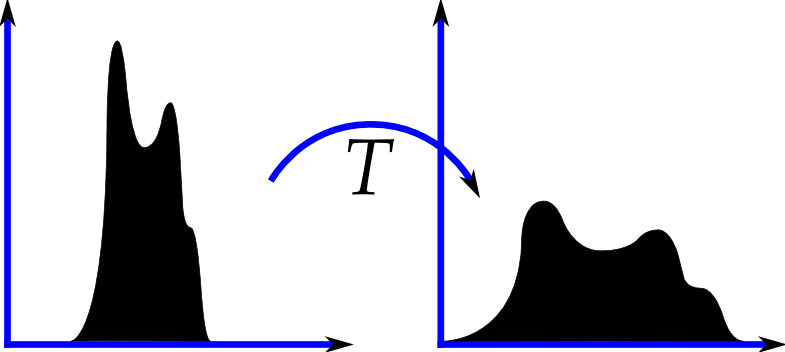
\includegraphics[width=0.5\textwidth]{img/histogram_equalization.png}
		\caption{Example of histogram equalization}		
		\label{fig:histeq}
	\end{figure}
		\subsubsection{The idea behind histogram equalization}
	[L] Our eyes (brain) can see more details if the image histogram is wide and approximately
	flat, rather than narrow and peaked.
	
	\subsubsection{Example: How to equalize a histogram in practice}
	[E] Assume you have a 2-bit image like this:
	\begin{equation}		
	\begin{bmatrix}
		1 & 1 & 2 & 2 \\
		2 & 1 & 3 & 1 \\
		1 & 1 & 0 & 1 \\
		1 & 2 & 2 & 1
	\end{bmatrix}
	\end{equation}
	\textbf{How do you equalize its histogram?}\\
	\\
	\textbf{Answer:} Create a table like table~\ref{tab:histeq}.
	\begin{table}[h!]
	\centering
	\begin{tabular}{lllll}
		\rowcolor[HTML]{EFEFEF} 
		Orig. Value & \multicolumn{1}{c}{\cellcolor[HTML]{EFEFEF}Probability} & Cum. prob. & Rounded & New Value \\ \hline
		0     		& $1/16$                                          		  & $1/16$     & $0/3$   & 0         \\ \hline
		1     		& $9/16$                                          		  & $10/16$    & $2/3$   & 2         \\ \hline
		2     		& $5/16$                                          		  & $15/16$    & $3/3$   & 3         \\ \hline
		3     		& $1/16$                                         		  & $16/16$    & $3/3$   & 3         \\ \hline
	\end{tabular}
	\caption{Histogram equalization table}
	\label{tab:histeq}
	\end{table}
	Then simply create the new equalized image by replacing the original values with the new values:
	\begin{equation}		
	\begin{bmatrix}
		2 & 2 & 3 & 3 \\
		3 & 2 & 3 & 2 \\
		2 & 2 & 0 & 2 \\
		2 & 3 & 3 & 2
	\end{bmatrix}
	\end{equation}
	This is the new equalized image. This histogram is poorly equalized due to small number of both
	bits and pixels.
	\subsubsection{Histogram equalization of a one-color image}
	Assume you equalize a histogram of an image of just one colour. As the probability will reach maximum
	at that gray value, the cumulative and rounded value will as well. Thus all original values will be 
	replaced with the maximum gray value (white).
	\subsection{Histogram matching}
	[W] Histogram matching is a method in image processing of color adjustment of two images using 
	the image histograms.\\
	\\
	It is possible to use histogram matching to balance detector responses as a relative detector 
	calibration technique. It can be used to normalize two images, when the images were acquired at 
	the same local illumination (such as shadows) over the same location, but by different sensors, 
	atmospheric conditions or global illumination.\\
	
	\subsubsection{Algorithm}
	[O] The algorithm is as follows. The cumulative histogram is computed for each dataset, see 
	figure~\ref{fig:histogram_matching}. For any particular value ($x_i$) in the data to be adjusted 
	has a cumulative histogram value given 
	by $G(x_i)$. This in turn is the cumulative distribution value in the reference dataset, namely $H(x_j)$. 
	The input data value $x_i$ is replaced by $x_j$. \\
    \\
    In practice for discrete valued data one does not step through data values but rather creates a 
    mapping to the output state for each possible input state. In the case of an image this would be a 
    mapping for each of the 256 different states. 
	\begin{figure}[h!]
		\centering
		\includegraphics[width=0.85\textwidth]{img/histmatch.jpg}
		\caption{Histogram matching diagram}		
		\label{fig:histogram_matching}
	\end{figure}
%	
%%%%%%%%%%%%%%%%%%%%%%%%%%%%%%%%%%%%%%%%%%%%%%%%%%%%%%%%%%%%%%%%%%%%%%%%%%%%%%%%%%%%%%%%%%%%%%%%%%%%%
%	
\section{Transform Functions}
\subsection{Basics}
A transform function, $t = f(\pi)$, transforms an input grey level $\pi$ into an output grey level t, for each pixel of the image.
\subsection{Types of transfer functions}
\begin{itemize}
\item Logarithmic: $t=log(1+\pi)$
\item Power-Law: $t=\pi^v$
\item Clipping: if $\pi \geq \pi_0$ then 1 else 0
\item Contrast strutching:
\end{itemize}

%	
%%%%%%%%%%%%%%%%%%%%%%%%%%%%%%%%%%%%%%%%%%%%%%%%%%%%%%%%%%%%%%%%%%%%%%%%%%%%%%%%%%%%%%%%%%%%%%%%%%%%%
%	
\section{Wavelets}
	\subsection{The fundamental Propertis of Wavelets}
	Wavelets are a multiscale method that can overcome some the difficulties with the Fourier Transform. Their fundamental
	property is to provide an adaptive time/space-frequency resolution to the the frequency itself [constant relative bandwidth, in the  
	language of data processing. In other words, this means that small-scale features of the data are analysed with fine resolution in
	time/space and coarse resolution in frequency, as is natural, and vice versa for large-scale features.
	 
	 \subsection{The Wavelet Transform}
	 TODO Maybe
	 
	 \subsection{Basics of Wavelet Applications}
	 Wavelets can be used for alot of things. Some common use-areas are:
	 
	 \subsubsection{Wavelet properties}
    [P04]
    \textit{Size of support} The support of a wavelet is the interval where the
    wavelet is non-zero. Its size determines not only the time/space localization 
    of the wavelet, but also the speed of the transform.\\
    \\
    \textit{Symmetry} also influences the quality of time/space localization. 
    For example, an asymmetric wavelet can be regarded as giving a location with 
    asymmetric error bars.\\
    \\
    \textit{Number of vanishing moments} A wavelet $\psi(x)$ has $n$ vanishing 
    moments when
    \begin{equation}
        \int_{-\infty}^\infty x^\upsilon \psi(x)dx=0, \mathrm{for }\;\upsilon = 0,1, \dots , n −1
    \end{equation}
    where x denotes time or space. In particular, all ‘normal’ wavelets have zero
    mean (n = 1) since, under rather general assumptions, this is related to the
    admissibility condition for the existence of the inverse transform. The number 
    of vanishing moments affects the frequency localization. In fact, the Fourier 
    transform of a wavelet with n vanishing moments peaks at a characteristic 
    frequency and decays as kn towards the origin, where k denotes frequency.\\
    \\
    \textit{Regularity} also affects the frequency localization. In fact, the 
    Fourier transform of a wavelet that is continuous together with its first 
    n − 1 derivatives decays as k−(n+1) towards infinity.\\
    \\
    \textit{(Bi-)Orthogonality} The orthogonality property concerns the set of 
    wavelets defining the transform, that is the set of scaled and trans- lated 
    versions of the basic wavelet. This means that such wavelets form an 
    orthogonal basis. The alternative bi-orthogonality property means that the
    decomposition and reconstruction wavelets form two distinct bases, which 
    are mutually orthogonal. Note that (bi-)orthogonality is intimately related
    to the non-redundancy of the transform.
	    
	    \subsubsection{Data Compression}
	    The adaptive time/space-frequency resolution and the non-redundancy of the fast wavelet transform have an iumportant implication: 
	    given regular data, most information present in the gets concentrated into a few large
	    wavelet coefficients. In practice, this means that we can set all the
	    other coefficients to zero and get back data almost identical to the
	    original ones. This is also the idea behind image compression. The most
	    important requirement for good compression ability is that the
	    decomposition wavelet should have many vanishing moments, and the basic
	    reason is that a wavelet with n vanishing moments is insensitive to
	    polynomials of degree n-1. 
	    
	    \subsection{De-noising}
	    The compression ability of the fast wavelet transform has a further
	    importan implication: given noisy data, the underlying regular parts gets
	    mostly mappen into many small wavelet coefficients, whereas noise is
	    mostly mappen into many small wavelet coefficients. In practice, this
	    means that, if we identify a correct threshold. then we can set all small
	    coefficients to zero and get back data almost decontaminated from noise.
	    This is the idea behind data denoising.
%	
%%%%%%%%%%%%%%%%%%%%%%%%%%%%%%%%%%%%%%%%%%%%%%%%%%%%%%%%%%%%%%%%%%%%%%%%%%%%%%%%%%%%%%%%%%%%%%%%%%%%%
%
\section{Image compression}
	\begin{description}
	    \item[Compression ratio] $C = b/L$, where $b$ and $L$ carries the same information, and
	    $L$ is the compressed data.
	    \item[Relative data redundancy] $1 - 1/C$
	    \item[Shannons entropy theorem (maximum compression rate)] $-\sum w_i \log_2 w_i$
    \end{description}
    \subsection{Redundancy types}
    [B]
        \subsubsection{Coding redundancy}
            A \emph{code} is a system of symbols (letters, number, bits and the like) used to
            represent a body of information or set of events. Each piece of information or 
            event is assigned a sequence of \emph{code symbols}, called a \emph{code word}.
            The number of symbols in each code word is its \emph{length}. The 8-bit codes that 
            are used to represent the intensities in most 2-D intensity arrays contain more
            bits than are needed to represent the intensities.
        \subsubsection{Spatial and temporal redundancy} 
            Because of the pixels of most 2-D intensity arrays are correlated spatially (i.e.,
            each pixel is similar to or dependent on neighboring pixels), information is
            unnecessarily replicated in the represintations of the correlated pixels. In an
            video sequence, temporally correlated pixels (i.e., those similar to or dependent
            on pixels in nearby frames) also duplicate information.
        \subsubsection{Irrelevant information} 
            Most 2-D intensity arrays contain information that is ignored by the human visual
            system and/or extreneous to the intended use of the image. It is redundant in the
            sense that it is not used.
    \subsection{Huffman coding}
        [W] See figure~\ref{fig:huffman}. A loss-less coding redundancy compression method.
        \begin{figure}[h!]
        \centering
        \includegraphics[width = 0.6\textwidth]{img/huffman_encoding.PNG}
        \caption{Huffman coding}
        \label{fig:huffman}
        \end{figure}
        \begin{equation}
            L = \sum_{i=1}^n w_i \cdot \mathrm{length}(c_i)
        \end{equation}
    \subsection{Run-length coding}
    Run-length encoding (RLE) is a very simple form of data compression in which runs of data (that
    is, sequences in which the same data value occurs in many consecutive data elements) are stored
    as a single data value and count, rather than as the original run. This is most useful on data 
    that contains many such runs. \\
    \\
    \textbf{Example:}\\
    The black and white image (displayed here as horizontal raster scanned):
    \begin{verbatim}
        WWWWWWWWWWWWBWWWWWWWWWWWWBBBWWWWWWWWWWWWWWWWWWWWWWWWBWWWWWWWWWWWWWW
    \end{verbatim}
    can be expressed as:
    \begin{verbatim}
        12W1B12W3B24W1B14W
    \end{verbatim}
        This is to be interpreted as twelve Ws, one B, twelve Ws, three Bs, etc.
        The run-length code represents the original 67 bit-values in only 18.
        RLE is loss-less.
        %
    \subsection{Description of lossy compression}
    [W] In information technology, "lossy" compression is the class of data encoding 
    methods that uses inexact approximations (or partial data discarding) for 
    representing the content that has been encoded. Such compression techniques are 
    used to reduce the amount of data that would otherwise be needed to store, handle,
    and/or transmit the represented content. The different versions of the photo of 
    the cat at the right demonstrate how the approximation of an image becomes 
    progressively coarser as more details of the data that made up the original 
    image are removed. The amount of data reduction possible using lossy compression can 
    often be much more substantial than what is possible with lossless data compression
    techniques.\\
    \\
    Using well-designed lossy compression technology, a substantial amount of data 
    reduction is often possible before the result is sufficiently degraded to be noticed 
    by the user. Even when the degree of degradation becomes noticeable, further data reduction 
    may often be desirable for some applications (e.g., to make real-time communication 
    possible through a limited bit-rate channel, to reduce the time needed to transmit the 
    content, or to reduce the necessary storage capacity).
    \subsection{Discrete Cosine transform}
    [W] The DCT, and in particular the DCT-II, is often used in signal and image processing, especially
    for lossy data compression, because it has a strong "energy compaction" property: most of the 
    signal information tends to be concentrated in a few low-frequency components of the DCT, 
    approaching the Karhunen-Loève transform (which is optimal in the decorrelation sense) for signals 
    based on certain limits of Markov processes. As explained below, this stems from the boundary 
    conditions implicit in the cosine functions.
    \begin{figure}[h!]
    \begin{align}
        X_{k_1,k_2} &=&
        \sum_{n_1=0}^{N_1-1}
        \left( \sum_{n_2=0}^{N_2-1}
        x_{n_1,n_2} 
        \cos \left[\frac{\pi}{N_2} \left(n_2+\frac{1}{2}\right) k_2 \right]\right)
        \cos \left[\frac{\pi}{N_1} \left(n_1+\frac{1}{2}\right) k_1 \right]\\ &=&
        \sum_{n_1=0}^{N_1-1}
        \sum_{n_2=0}^{N_2-1}
        x_{n_1,n_2} 
        \cos \left[\frac{\pi}{N_1} \left(n_1+\frac{1}{2}\right) k_1 \right]
        \cos \left[\frac{\pi}{N_2} \left(n_2+\frac{1}{2}\right) k_2 \right] .
    \end{align}
    \caption{Multi-dimensional discrete cosine transform}
    \end{figure}
    
    \subsection{Compression of JPEG}
    [W] JPEG uses a lossy form of compression based on the discrete cosine 
    transform (DCT). This mathematical operation converts each frame/field 
    of the video source from the spatial (2D) domain into the frequency 
    domain (aka transform domain.) A perceptual model based loosely on the 
    human psychovisual system discards high-frequency information, i.e. 
    sharp transitions in intensity, and color hue. \\
    \\
    In the transform domain, 
    the process of reducing information is called quantization. In simpler 
    terms, quantization is a method for optimally reducing a large number 
    scale (with different occurrences of each number) into a smaller one, 
    and the transform-domain is a convenient representation of the image 
    because the high-frequency coefficients, which contribute less to the 
    overall picture than other coefficients, are characteristically small-
    values with high compressibility.\\
    \\
    The quantized coefficients are then 
    sequenced and losslessly packed into the output bitstream. Nearly all 
    software implementations of JPEG permit user control over the 
    compression-ratio (as well as other optional parameters), allowing the 
    user to trade off picture-quality for smaller file size. In embedded 
    applications (such as miniDV, which uses a similar DCT-compression 
    scheme), the parameters are pre-selected and fixed for the application.
%	
%%%%%%%%%%%%%%%%%%%%%%%%%%%%%%%%%%%%%%%%%%%%%%%%%%%%%%%%%%%%%%%%%%%%%%%%%%%%%%%%%%%%%%%%%%%%%%%%%%%%%
%	
\section{Usefull formulas}
    \subsection{statistics}
        \subsubsection*{Mean, $\overline{X}$ or $\mu$}
            \begin{figure}
\[ \overline{X} = \frac{\sum{X}}{N} \]
\caption{$X$ : all samples, $N$ : number of samples}
\end{figure}
            \
            
            For random variables the mean is the \textit{expected value}.
            \begin{figure}
\[ E[X] = \sum^{\infty}_{i=1{x_ip_i}} \]
\caption{$E[X]$ : ezpected value, $x_i$ : a event $i$, $p_i$ : probability of event $x_i$}
\end{figure}
        \subsubsection*{Variance, $\sigma^2$}    
         
         

        [w]In probability theory and statistics, variance measures how far a set of numbers is spread out. A variance of zero indicates that all the values are identical. Variance is always non-negative: a small variance indicates that the data points tend to be very close to the mean (expected value) and hence to each other, while a high variance indicates that the data points are very spread out around the mean and from each other.
        
    \subsection{Histograms}
    
    \subsection{Flux}
        flux = intensity\\
        $\mu = \frac{\text{flux}}{\text{img size}}$
    
\section{Old exams}
    \subsection*{2014-10-30}
    \subsubsection*{1a)}
        Most important assumptions for Wiener filtering is: 
    \begin{itemize}
        \item{1: the noise is additive.}
        \item{3: the noise is uncorrelated with the signal.}
    \end{itemize}
    
    \subsubsection*{1b)}
        Answer is in lecturenotes \textit{Image restorations 2}
        obs: $H = 1$, since no distortions\\
    
    \subsubsection*{1c)}
        Referring to:
        $G = F + N$, thus noise needs to be additivit.
        Also for wiener filter the powerspectrum of G must be as: \\    
        $<|G^2|> = |F^2| + <|N^2|> + <FN^*> + <F^*N>$
    If noise is corralated with the signal then:\\
    $F \bigstar N \neq FN$ \\

    \subsubsection*{1d)}
        Speckle noise: uniform, multiplicative, noise.\\
        Make noise additive by taking the logarithm of the image. Afterwards it's possible to do the noise reduction since the noise is uncorraleted with the image.\\ 
        \textbf{Obs}: introduce a bias $\epsilon$ when taking logarithm, since $\log{0}$ is not defined.\\
        \textbf{Obs}: Logarithm-function is not linear, that means that the total \textit{Flux} is not conserved. It can be adjusted by calculating the total \textit{flux} before the logarithmic operation, and in the post-processing step(when the exponential-function is run). Divide the \textit{flux} by total amount of pixels in the image to calculate the mean. This is the bias. Subtract the bias from the wienerfiltered image. Otherwise the resulting image contains errors. (OBs, this is taken from my notes, Im not sure this is the correct way of calculating the bias).
        
        \subsubsection*{1e)}
        Poissionian: not additiv, correlated with the image.
        \\
        Both assumptions are violated.
        There is a transformation, the Anscombe Transformation, that can be applied to the image, wich makes the poissionian noise to an approximately signal-independent Gaussian additive noise. Which can be wiener filtered. 
    \subsubsection*{1f)}
    Salt-And-Pepper: not additive \\
    no transformation to becom additive \\
    Cant use wiener filter.
    
    \textbf{super-poissonin-noise is a wrong answer}. Since super-poissonin-noise only appear in the power spectrum, not in the spatial domaine.
        
    \subsubsection*{2a)}
    Given two versions of same image \textit{I1} with sample size 16x16 pixels and \textit{I2} with sample size 1024 x 1024 pixels. We can precompress \textit{I2} more since we can traverse more levels using a wavelet. A wavelet stops when the whole image is in the spectra.\\ 
    ex:\\
    \begin{itemize}
    \item level 1: wavelet size
    \item level 2: $2 \cdot$ level 1
    \item level 3: $2 \cdot$ level 2
    \item ...
    \end{itemize}
    
    The more levels that can be traversed, more sigingicant data can be concentrated into large wavelet coefficients, which means more unneccesary coefficients can be set to zero. Thus a larger sample size gives a better pre comression.
    
    \subsubsection*{2b)}
    Given from question: \\
    Using wavelet \textit{bior4.4} \\
    support size: 12px \\
    significant difference: 3px\\
    Image size, \textit{I1}: 16x16\\
    Image size, \textit{I2}: 1024x1024\\
    
    First choose wich level,$\ell$, to stop at using function:\\
    $2^{\ell-1} \cdot \text{wavelet-size} \approx \text{image size, in min dimension}$
    
    For \textit{I1}\\
    $2^{1-1}\cdot 12 \approx 16 \rightarrow \ell = 1 \text{for \textit{I1}}$\\
    For \textit{I2}\\
    $2^{7-1}\cdot 12 = 64 \cdot 12 \approx 1024 \rightarrow \ell = 7 \text{for \textit{I2}}$
        
    The difference betwen wavelets coeficiance is: $\frac{2^7}{2^1} = 2^6 = N_a$\\
    
    upperlimit :=$ N^2/N_a $\\
    upperlimit \textit{I1} :=$ 16^2/ 2^6 = 2^2$\\
    upperlimit \textit{I1} :=$ 1024^2/ 2^6 = 128^2$\\
     
     
     Since wavelet only is significant, wich means theese $3px$ will have the most inpact on the compression. We can use $3px$ as wavelet-size instead of $12px$, and redo the calculations.
     wich gives us: \\
     $\ell = 3 \text{for \textit{I1}}$ \\
     $\ell = 9 \text{for \textit{I2}}$ \\
     
     Wich yield a $N_a=2^2$
     
     OBS: IM NOT SURE THIS ANSWEAR IS RIGHT!!!!!!
     
     \subsubsection*{2c)}
     Given:\\
     Img size: $128 \times 128$ px\\
     color: $8$-bit\\
     Distrubution: Guassian\\
     $\sigma= 16$\\
     $\mu= 64$\\
     
     \begin{itemize}
    \item 8-bit $\rightarrow 255$ Distinct gray-Values
    \item $\mu < 127 \rightarrow$ Image is dark, since most values are distrubuted in the darker part of the histogram. 
    \item $\sigma << 255 \rightarrow $ values are close to eachother, thus low contrast
    \end{itemize}
    
    The flux is define as the total intensity of the image. And mean is defined as total intensity over all pixels. Thus:
    
    flux = intensity\\
    $\mu = \frac{\text{flux}}{\text{img size}} \rightarrow $\\
    flux = $128^2 \cdot 64$
    
    \subsubsection*{2d)}
    Since the $\sigma$ is $< 10$. The \textit{poissonan distrubution} can be treated as a \textit{guassian distrubution}. Same calculations used in assignment 2c can be applied but with the new given values.
    
	\subsection{2014/2013}
	\subsubsection*{1a)}
	
	    Sharpened image = Original image - smoothened image.\\
	    You can smoothen an image by taking a lowpass filter. 
	
	\subsubsection*{1b)}
	
	    Amplify high frequency components while keeping the low frequency intact. This will enhance images and remove some blurry parts. \\
	    High boost image = Original image + Sharpened image. 
	    \\By 1a).
	
	\subsubsection*{1c)}
	
	    For instance use: The Laplacian of gaussian method. Works by looking for zero-crossings after filtering the image with the Laplacian of a gaussian filter
	
	\subsubsection*{1d)}
	
	    Yes. By amplifying high frequencies we can sharpen an image and by looking at high frequencies we can find edges.
	
	\subsubsection*{1e)}
	
	    Finns i facit.
	    
	\subsubsection*{2a)}
	
	    TODO
	    
	\subsubsection*{2b)}
	    Denoising: W3 because it looks like the reconstruction wavelet, behaves more than W2 like an orthogonal 
	    and has more vannishing moments than the orthogonal.\\
	    \\
	    Wavelets are good for additive white gaussian noise so yes.\\
	    \\
	    If not Gaussian, preprocess and map into white-gaussian.\\
	    \\
	    For salt and pepper noise you can not use wavelets, need to use a median filter.
	    
\subsection{2012/2013}

    \subsubsection*{1a)}
    
        A basic noise model used to mimic the effect of many random processes that ocure in nature. \\
        Additive - Because it is added to any noise that might be intrinsic to the information system.\\
        White - Has uniform emissions at all freq in the visible spectrum.\\
        Gaussian - Because it has a normal distribution in the time domain with an average time domain value of zero.\\
        Can be removed using (adaptive) median filters or linear filtering.
        
    \subsubsection*{1b)}
    
        Poissionian Noise is a type of electrical noise originating from the discrete nature of electric charge. 
        Gaussian noise is continious were as poissonian noise is discrete. Poissonian noise can occure in TV-streams. \\
        To remove Poissonian noise, maybe use an averaging filter because the noise is statistic.
        
    \subsubsection*{1c}
    
        By denoising we remove information from the image, which means we're compressing it.
        
    \subsubsection*{}
        
        Exists facit for the rest
        
\subsection{2011/2012}

    \subsubsection*{1a)}
    
        It can be used to change contrast. By taking the histogram and removing peeks, and stretch the rest, we get higher contrast.
        (stretching the gray scale)
    
     \subsubsection*{1b)}
     
        Can be used for color adjustment and gray scale adjustment (not just by histogram equalize).
        
    \subsubsection*{1c)}
    
        Low-pass filter passes signals under a certain cut-off frequencies. All freq above is dampened but not necessary removed. 
        Ideal filter completely eliminates all above cut-off freq. Can be used against wide-random noise. (maybe same thing as additive
        gaussian noise?)\\
        \\
        Cons: Ideal filter will remove all high freqs, which means that all edges will be smoothened.\\
        \\
        Pros: Good if you don't have many distinct edges, because it can remove a lot of high freqs. 
        Not used so much in image processing but rather in aduio processing, where you want to completly 
        remove certain freqs (above a certain freq).
        
    \subsubsection*{1d)}
    
        Works pretty much the same way but not ideal so wont remove all freqs above cut-off freq.
        
    \subsubsection*{}
    
        Resten har facit.
        
\subsection{2010/2011}

    \subsubsection*{1a)}
        
        Averaging filter works as a mean-filter.
        
    \subsubsection*{1b)}
        
        It will work better with a median filter.
        
    \subsubsection*{3c)}

        Helps to remove blur. Optimal means optimal in the sense of MMSE, minimum mean square error.
        
        TODO

    \subsubsection*{}
    
        Resten har facit. 
        
\subsection{2009/2010}

    \subsubsection*{1a)}
    
        Trivialt ordbajs.
    
    \subsubsection*{1b)}
    
        When enhancing the lower frequencies or dampening the high frequencies. Threseholding is the simplest
        method of image segmentation. Can be used to create binary images from a gray scale image. 
        All pixel values (A) to the left of the centered line (B) will be white, and all to the right (C), will be black.
        \begin{verbatim}
                 ______________
                |
                |
  ______________|
    A     <     B     <     C
            
        \end{verbatim}

    \subsubsection*{1cde)}
    
        Finns facit. Det som inte finns facit på skulle han inte ta med.
        
    \subsubsection*{2c)}
    
        FWT (Fast Wavelet Transform)\\
        \textbf{Pros:} Good ability to compress stationary signals, able to support some interesting noneucledian similarity measures.\\ 
        \textbf{Cons:} Signals must have length: $2^{INT}$. Can't support weighted distance measures.\\
        \\
        BDCT (Block discrete cosine transform)\\
        Better at comparisons. The difference from FWT is that it takes real cosine functions instead of a set of harmonicaly related complex
        exponential functions like the DFT. Specially used for lossy data compression because of it's strong energy compaction property. 
        Good and bad.\\
        \\
        DFT (Discrete Fourier Transform)\\
        Good for same things as BDCT, namely Lossy image compression.\\
        \textbf{Pros:} Good ability to compress most natural signals. Fast $\mathcal{O}(n \cdot \log(n))$. 
        Weekly abeled to support timewarped queries. \\
        \textbf{Cons:} Difficult to deal with sequences of different lengths. Can't support weighted distance measures.
        
\subsection*{2008/2009}

    Finns facit på allt.
\end{document}